\chapter{Research}
With the writers lack of experience in writing applications of this type, the research phase explored a number of different avenues and began with very little in terms of preconceptions. 

\section{Similar Applications}
Initial focus was directed towards exploring existing applications that performed a similar task to gain some insight as to the expectations of the project. A number of applications that provide recognition from input devices such as the camera, microphone and other peripherals were examined.

\colorbox{red}{Three classes of application server, client/server, client only discussed below}

\subsection{Google Goggles}
With the release of the Android operating system Google have been exploring a number of user interaction mechanisms for the system. Of these alternative approaches they have had much success with the impressive \textbf{Google Voice Search}, which enables the user to command the device using their voice without any form of training.

Google have also invested resources into the development of a visual search system which they call \textbf{Goggles}. Just like Voice Search, Goggles performs very little processing on mobile handset, instead opting to transmit the data to a back-end service for processing.

Due to the commercial and proprietary nature of the product implementation details are hard to come across, but in August 2010 Google delivered a presentation at the Hot Chips conference in Stanford University that gives insight into some elements of the design of the service. During this talk Google discussed a number of interesting points, firstly due to level of processing involved and network latencies on current generation cellular networks a image search query takes in the region of about 6.5 seconds for the system to return a result to the handset. Google also broadly discussed the architecture of the back-end search processing, when an image is received by the remote server it is in parallel analysed by a number of engines. Each of these engines are tuned for extracting particular information from an image, for example they have a barcode, text, landmark, wine label and logo engine to name a few, currently it is estimated that a search is executed on 20 engines in parallel and each result is ranked with only the most confident being returned to the user \cite{vbgoggles10, sbs10}.

\begin{figure}[h!]
\centering
    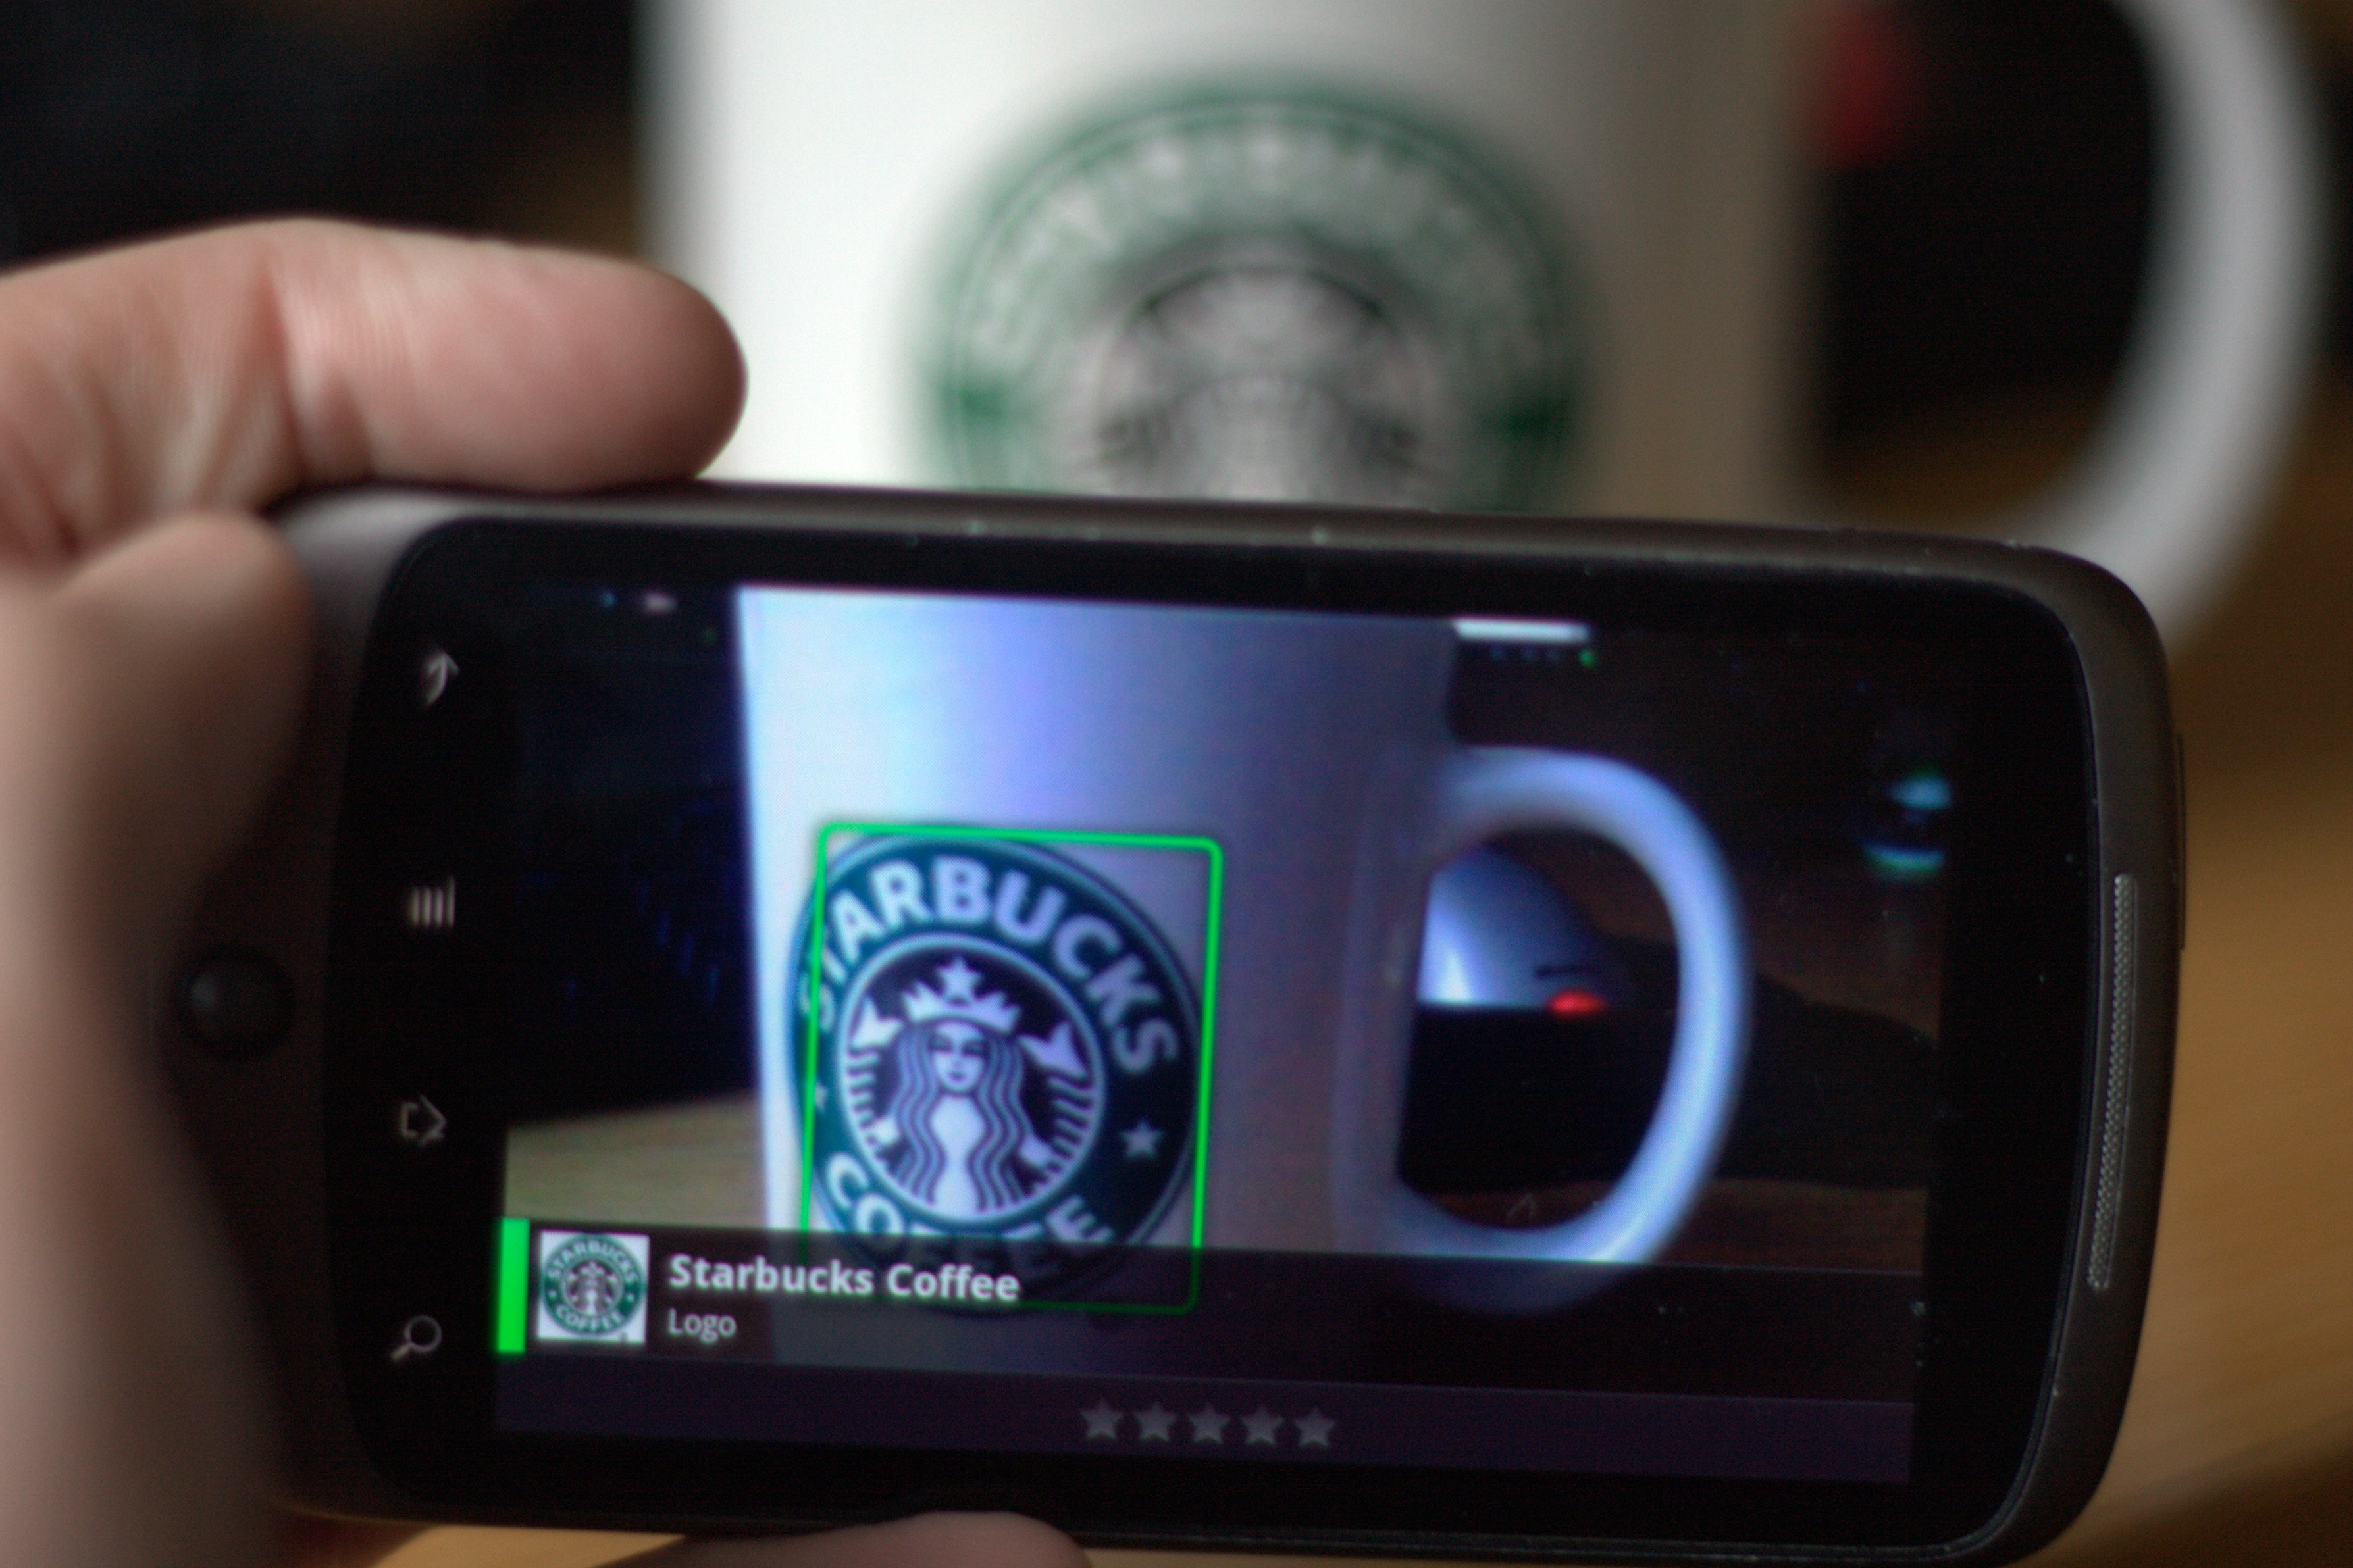
\includegraphics[width=0.7\textwidth]{research/images/goggles_example.jpg}}
	\caption[Google Goggles example]%
    {Google Goggles successfully identifies a well known logo from a coffee mug.}
\end{figure}

Google presented at the Hot Chips conference to raise awareness of the necessity to maximise the amount of processing done in the device to chip manufacturers in order to counter the latency inherent in cellular networking.

Interestingly they also discussed the use of data from other sensors to increase the context of the image, for example including geographical coordinates with an image of the Eiffel Tower could potentially aid in a more speedy result being returned.

Goggles is not currently successful at identifying instances of particular classes of objects. In their documentation they specifically mention not having a high success rate when recognising objects such as tree leaf types, animals or cars. Another major drawback is the estimated 6.5 second average response time, but this is largely bourne from transmitting the unprocessed image over the network which encompasses issues out of the control of device makers.

\subsection{Shazam}

While on initial review it may seem that Shazam is unrelated to the current project, a closer inspection reveals many similarities. Shazam is a application and back-end service which allows its users to identify a piece of music based on a short sample potentially recorded in a noisy environment with a sub-par microphone.

The application records an audio sample, performs local processing to generate a fingerprint and then performs a remote lookup against a database for the artist and song title. It is necessary to perform these remote lookup’s due to the size and proprietary nature of Shazam’s music database. Transmitting only the fingerprint minimises the bandwidth consumed and requires much less processing facility on the server side \cite{wang03}.

\colorbox{red}{The "acoustic fingerprints" used by Shazam are based on spectrogram data representing time, frequency, and intensity}

Although processing audio data instead of image data, this system has many common elements with the architecture being investigated for this project. Commonalities conceivably include:

\begin{enumerate}
\item Client/Server Architecture of the system.
\item Searching and sorting of a large database of fingerprints.
\item Fingerprinting of data from a sensor.
\end{enumerate}

As this is again a commercial product and we are limited in the information we can uncover relating to its operation. Although somewhat more information is available when compared to Google Goggles due to its founders publishing a paper relating to the design of the audio fingerprinting algorithm and a number of documents existing about the design of such software.

\subsection{ZXing Barcode Scanner}
The final application analysed at this stage of the research is the ZXing Barcode Scanner which is based on the ZXing open-source multi-format barcode image scanning library \cite{zxingproject}. This application is capable of scanning all major bar-code types including UPC, EAN and QR on the mobile handset without network connectivity.

When the application is started the user is presented with an on screen view finder for the camera which has a horizontal red line to help the user place the camera in the correct location for scanning UPC or EAN codes. When the software correctly focuses the camera it automatically recognises any valid bar-codes and proceeds to display the encoded data in a way valid for the type of bar-code. The user is presented with a number of options based on the type of code just scanned, for example if a UPC ISBN code has been scanned a button is displayed to search for the book online we see an example of this in Figure \ref{zxing_scanner}.

\begin{figure}[h!]
\centering
    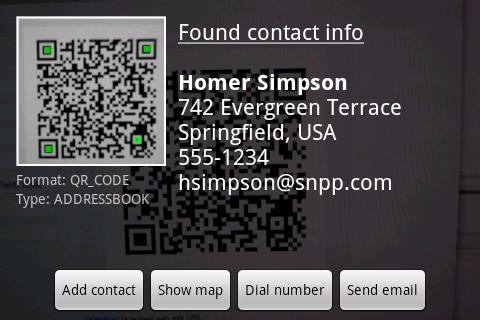
\includegraphics[width=0.6\textwidth]{research/images/zxing_barcode.jpeg}
	
	\caption[ZXing Barcode Scanner]%
    {ZXing Barcode Scanner displaying the result of scanning a QR Code containing contact details.}
	\label{zxing_scanner}
\end{figure}

It is valuable to identify an application at this stage that is capable of performing some form of image analysis on the handset. While the application of the image analysis in this instance is being applied to relatively structured input it is still faced with performance, lighting and optical constraints that are likely to play a factor in this project.

\section{Android Platform}
As mentioned earlier in this report, the Google Android platform has gained considerable market penetration in the short few years since its release in 2008. A large number of manufacturers including Samsung, LG, Motorola, HTC and Sony Ericsson have been producing Android based handsets at a vast range of price points and configurations. This variety of available hardware coupled with development for the platform through the Java programming language makes it an appealing platform to develop for.

Android is an open-source software stack designed for mobile devices it is developed by Google and the Open Handset Alliance and is maintained by the Android Open Source Project (AOSP). It consists of a modified Linux Kernel, Android Runtime also known as the Dalvik virtual machine, Libraries, Application Framework and a collection of Applications.

\subsection{Architecture}
\subsubsection{Kernel}
Android at its lowest level utilises a Linux 2.6 based kernel, listed below are some of the more major modifications \cite{elinuxandroidkernel}. Due to the level of modification, specifically changes to locking, the security model and the driver infrastructure this Android code is not part of the mainline kernel \cite{registerAndroidKernel10}. It is important to note that in the Android environment does not provide support for the full set of standard GNU libraries with glibc being a prime example, this may provide difficulty when porting projects to the environment.

\begin{itemize}
\item IPC - Addition of CORBA-like IPC mechanism (Binder)
\item Shared memory allocator (ashmem)
\item Process memory allocator (pmem)
\item Logging - Support for Android logcat command
\item Power management (wakelocks) 
\item OOM - Out of memory handling modifications
\end{itemize}

As we can see in Figure \ref{android_arch} the kernel provides core systems services such as memory, process, power and network management as well as abstracting the hardware away from the rest of the stack.

\subsubsection{Native Libraries}
Moving up the stack to the libraries section, Android provides a number of C/C++ based libraries which can been seen in Figure \ref{android_arch}. Much system wide functionality is implemented here, for example Surface Manager which manages the display subsystem and SQLlite which provides structured storage to installed applications. Also interestingly the web-browser rendering engine is provided as a library/service at this level which is done to enable as fast as possible rendering of content \cite{googioanatomy08}. 

\colorbox{red}{Should I expand on the difference between services/libraries at this stage and Kernel Space/User Space}

\colorbox{red}{Boot Process \url{http://elinux.org/Android_Booting}}

\begin{figure}[h!]
\centering
    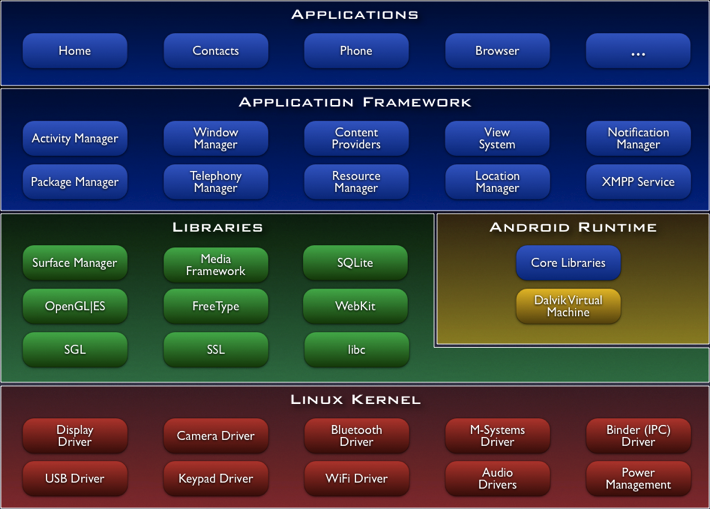
\includegraphics[width=1\textwidth]{research/images/android_arch.png}
    \caption{Android architecture overview}%
    \label{android_arch}
\end{figure}

\subsubsection{Virtual Machine}
Illustrated differently in Figure \ref{android_arch} but at the same level in the stack is the Dalvik JIT based process virtual machine and Harmony open-source Java class library. The Dalvik virtual machine is a crucial element is the Android stack, on-top of which all user facing code is executed.  The use of such a virtual machine enables the development of applications in a memory managed environment. Additionally as it is a process based virtual machine each process starts its own instance of the VM and depends on the system kernel for threading and low level memory management. In the case of a crashed or hung application the VM can be terminated without effect on other running applications or services.

Dalvik is different from traditional VM’s in that it is register based and not stack based like the Java Virtual Machine. This register based approach uses in the region of 47\% less instructions but the executable size tends to be larger \cite{ehringerdalvik10}.

The Android developers have attempted to mitigate this larger executable size by create a new executable file format called dex. In a traditional Java application each class is compiled into a bytecode .class file and these files are zipped up to build a .jar file. When building an Android application these .class files are compiled into a single .dex executable. This enables space savings to be made by sharing data like literal constants and headers that would normally be duplicated across a number of .class files \cite{ehringerdalvik10}.

This register based approach with dex format executable’s is optimised for battery based devices with constrained CPU and memory. 

It is important to note that the Java Implementation does not utilise all of the established Java standards (Java SE, Java ME), which prevents compatibility among Java applications written for other environments.

\subsubsection{Application Framework}
The last level of the Android platform we are going to explore is the Application Framework seen in Figure \ref{android_arch}. This framework is a set of Java based API’s which give developers access to all the services and libraries listed in the previous sections. It is also important to note that developers have access to the same framework API’s that are used by core applications such as the Dialer and Text Messaging applications.

The API is divided into a number of discrete units of functionality, each of these can be seen in the architecture overview diagram. A developer may not interact directly with many of these components but they form the basis for the framework.

Below we will briefly describe some of the key framework components.

\begin{description}
\item[Activity Manager] Manages the applications lifecycle (Started, Running, Background, Killed) and notifies your application when the phone is about to move from one state to the next. The Activity Manager also maintains a common stack enabling a user to navigate from one application to another seamlessly.
\item[Resource Manager] Contains all the infrastructure to manage strings, layouts and bitmaps for different locals and screen resolutions.
\item[Location Manager] Provides geographic location data to an application. This provides access to hardware GPS devices as well as less accurate location data from services such as Skyhook.
\item[Notification Manager] Offers a number of methods to notify the user of an event, this can include displaying icons, flashing LED’s, vibrating or playing a sound.
%less important for developers
\item[Window Manager] Creates surface’s onto which the application may draw its UI (View).
\item[Content Providers] Special types implemented by the system or by applications to enable data sharing across applications, common content providers include contacts, media store and call log.
\item[View System] Provides a the infrastructure for building user interface components (buttons, text boxes etc.) and their associated event handling. The view system provides access to the components in a tree like structure, much like the HTML DOM concept.
\item[Package Manager] Enables access to various kinds of information about packages (applications) installed on the system.
\item[Telephony Manager] Provides information to an application about the current state and availability of telephony services on the device. 
\end{description}


\subsection{Application Structure}

Android applications are packed into an APK file, which essentially a collection of components that share a set of resources such as databases, file space and preferences as well as a Linux process \cite{googioappframework08}. Each of these components has a managed filecycle which is controlled by the Activity Manager.

Android applications are a collection of Activities, Tasks and Processes this structure is illustrated in Figure \ref{activity_activities_tasks_processes}. An activity is regarded as a single concrete element of functionality which may not have any UI, where as a task is a collection of activities potentially across a number of applications which are used to complete some unit of work. This offers the developer the ability create new applications that can to knit together existing components to maximise reuse and minimise development time.


\begin{figure}[h!]
\centering
    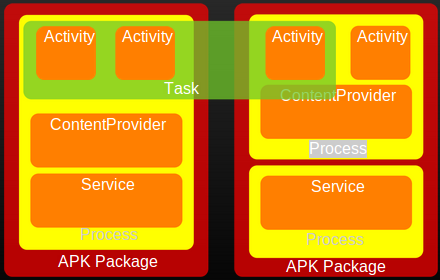
\includegraphics[width=0.55\textwidth]{research/images/activities_tasks_processes.png}
    \caption{Android Activities Tasks and Processes}%
    \label{activity_activities_tasks_processes}
\end{figure}

As we have seen Android application framework is heavily designed around the concept of components, this component model incorporates:

\begin{itemize}
\item Activity Components\\
Often represented as a single screen but may also have no UI, and is regarded as a focused element of functionality. Each activity has its lifecycle managed by the Activity Manager as illustrated in Figure \ref{activity_lifecycle}.
\item Service Components\\
Used typically when some long-run task is required, they have no UI and will run indefinitely. These services may be started by an Activity, but they continue to run after the Activity has been closed.
\item Intent Receiver Components 
Listens for broadcast Intents and performs some action. These Intents may be broadcast by the system e.g. battery low, notify the arrival of a message etc. or Intents may originate from other applications to signify some change of state.
\item Content Provider Component\\
Provides specific data in your application to other applications, not generally used to share data within an application.
\end{itemize}


\begin{figure}[h!]
\centering
    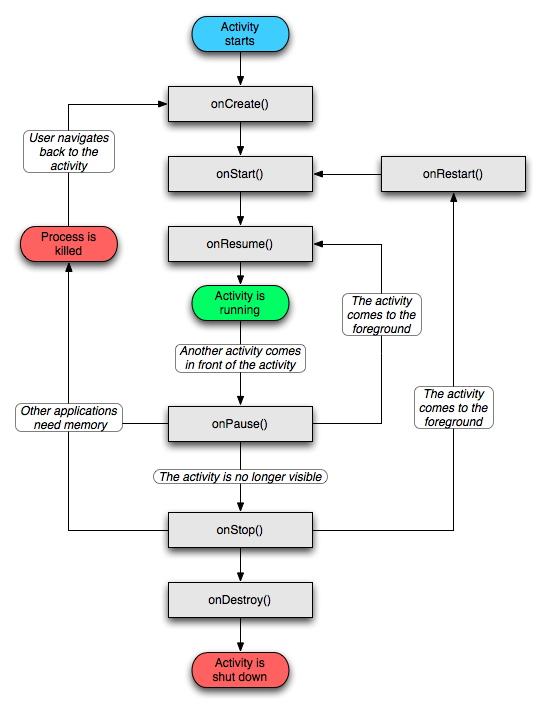
\includegraphics[width=0.7\textwidth]{research/images/activity_lifecycle.png}
    \caption{Android Activity Lifecycle}%
    \label{activity_lifecycle}
\end{figure}

\subsection{Development Enviroment}


To begin developing an understanding of the platform a number of tutorials and documents on the developer site \url{developer.android.com} were followed, and they proved to be valuable in getting to grips with the platform. 

\section{Computer Vision}

\subsection{Libraries}

\subsection{Techniques}

\section{Focus}
